\documentclass[a4papaer]{article}
\usepackage[pdftex]{graphicx} 
\usepackage{enumitem}
\setdescription{leftmargin=\parindent,labelindent=20mm}

\title{{\bf Medical Store Management System}\\Phase-2}
\author{Shikhar Sharma\\10682\\shikhars@iitk.ac.in\\\\CS315 Course Project\\IIT Kanpur}

\begin{document}

\maketitle
\tableofcontents

\newpage
\section{Extended Entity-Relationship Model}
The Extended Entity-Relationship Model for the project is given below:\\
\hspace*{-30mm}
{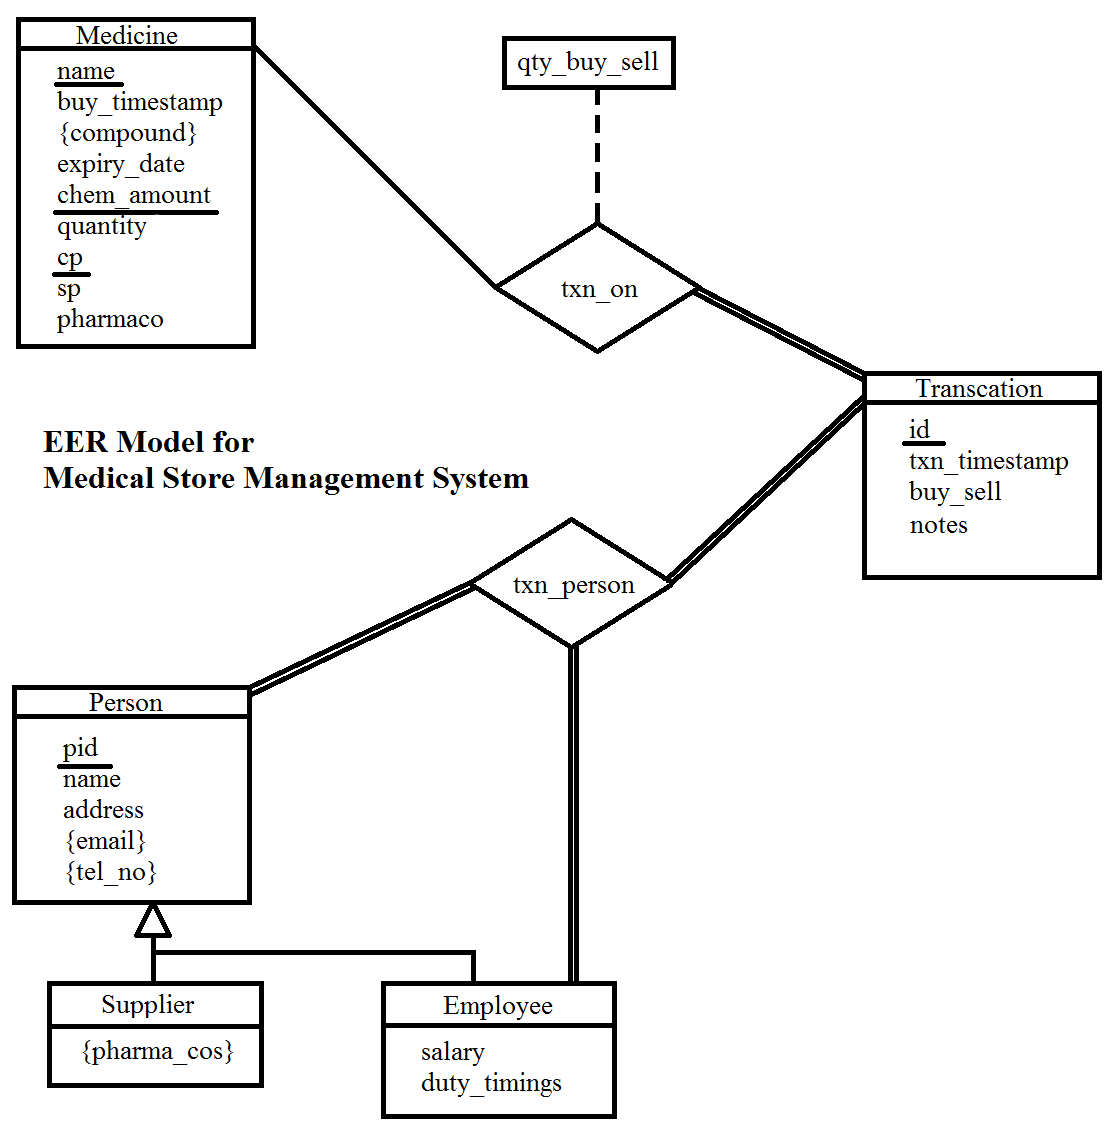
\includegraphics[width=180mm]{eerd.png}

\section{Details}
\subsection{Constraints}
In the Entity-Set {\bf Medicine}, PRIMARY KEY is (name,chem\_amount,cp).\\\\
In the Entity-Set {\bf Transaction}, PRIMARY KEY is (id) which is generated by auto-increment.\\\\
In the Entity-Set {\bf Person}, PRIMARY KEY is (pid) which is also generated by auto-increment.\\\\
Total participation has been indicated in the EER Model by drawing double lines.\\\\
The specialization of Person into Supplier and Employee is a disjoint specialization which is partial.

\subsection{Domain Types}
\begin{description}
		\item[name] varchar(60)
		\item[buy\_timestamp] timestamp
		\item[compound] varchar(50)
		\item[expiry\_date] date
		\item[chem\_amount] varchar(10)
		\item[quantity] int
		\item[cp] int
		\item[sp]int
		\item[pharmaco] varchar(50)
		\item[qty\_buy\_sell] int
		\item[id] int
		\item[txn\_timestamp] timestamp
		\item[buy\_sell] char(1)
		\item[notes] text
		\item[pid] int
		\item[name] varchar(60)
		\item[address] text
		\item[email] varchar(45)
		\item[tel\_no] int
		\item[pharma\_cos] varchar(50)
		\item[salary] int
		\item[duty\_timings] varchar(20)
	\end{description}

\subsection{Multiplicities}
A Transaction will have only one Person and one Employee involved. Except for this relation, every other relation in the EER Model is many-many.

\end{document}